%-------------------------------------------------------------------------------
%	CHAPTER 4
%-------------------------------------------------------------------------------

\chapter[Straight lines]{Straight lines are shortest paths}
\label{ch:straight-lines}

We now turn to optimisation problems over infinite-dimensional spaces (spaces of functions or paths). For example:
\begin{itemize}
\item minimising the length of a path between two points,
\item minimising the surface tension of a soap film,
\item minimising the length of a loop which encircles a given area.
\end{itemize}
The idea is to consider (for example) the length functional as a function on the space of paths and to find its critical points. This is called the calculus of variations. We illustrate it in this lecture by proving:

\begin{thm}
A straight line is the shortest path between two points in the plane.
\end{thm}
Recall (see \url{http://youtu.be/bM_klC-oAzg}) that the length of a smooth path $\gamma\colon[0,1]\to\RR^2$ is the integral
\[\int_0^1|\dot{\gamma}(t)|dt.\]
If $\gamma(t)=(x_1(t),x_2(t))$ in coordinates then this is just
\[\int_0^1\sqrt{\dot{x}_1^2+\dot{x}_2^2}dt.\]

\section{Proof}

We will prove the theorem in two stages.
\begin{enumerate}
\item We introduce the {\em action} of a path,
\[A(\gamma)=\int_0^1|\dot{\gamma}(t)|^2dt\]
which is something like the kinetic energy of the path. We have
\[\left|\int_0^1|\dot{\gamma}|dt\right|^2\leq\int_0^1|\dot{\gamma}(t)|^2dt\]
by the Cauchy-Schwarz inequality, with equality if and only if $|\dot{\gamma}(t)|$ is constant. Now we can always reparametrise a path so that $|\dot{\gamma}(t)|$ is constant (just move along the path with constant speed $L(\gamma)$). Reparametrising a path does not change its length. The outcome of this argument is that {\em it suffices to show that a straight line minimises action}.
\item Now we have to prove:
\end{enumerate}
\begin{prp}
A straight line minimises the action integral
\[\int_0^1\left(\dot{x}_1^2+\dot{x}_2^2\right)dt\]
amongst all smooth paths between two points in the plane.
\end{prp}
\begin{proof}
Let $\gamma\colon [0,1]\to\RR^2$ be the straight line connecting the two given points, parametrised with constant speed $L(\gamma)$ and write $\gamma(t)=(\gamma_1(t),\gamma_2(t)$. Suppose that $\delta$ is another path joining the two given points and write $\delta(t)=(\delta_1(t),\delta_2(t))$. Define $\epsilon_i(t)=\delta_i(t)-\gamma_i(t)$ ($i=1,2$) so that we can write $\delta=\gamma+\epsilon$. Since both paths have the same endpoints, $\epsilon(0)=\epsilon(1)=0$.

Now
\begin{align*}
A(\delta)&=\int_0^1|\dot{\delta}|^2dt\\
&=\int_0^1\left(|\dot{\gamma}|^2+|\dot{\epsilon}|^2+2\dot{\gamma}\cdot\dot{\epsilon}\right)dt\\
&=A(\gamma)+A(\epsilon)+2\int_0^1\dot{\gamma}\cdot\dot{\epsilon}dt
\end{align*}
Since $\dot{\gamma}$ is constant (it is the tangent vector to a straight line) this final integral is
\[2\int_0^1\dot{\gamma}\cdot\dot{\epsilon}dt=2\dot{\gamma}\cdot\int_0^1\dot{\epsilon}dt\]
which is
\[2\dot{\gamma}\cdot(\epsilon(1)-\epsilon(0))\]
by the fundamental theorem of calculus. This vanishes because $\epsilon(0)=\epsilon(1)=0$. Thus
\[A(\delta)=A(\gamma)+A(\epsilon)\]
which is greater than or equal to $A(\gamma)$ with equality if and only if $\delta=\gamma$ because $\int_0^1|\dot{\epsilon}|^2dt\geq 0$ with equality if and only if $\dot{\epsilon}=0$, if and only if $\epsilon(t)=\epsilon(0)=0$ for all $t$.
\end{proof}

\section{Dissecting the proof}

This proof worked so well because the problem was so simple. Most variational problems do not have nice easy solutions like straight lines. We will abstract the key ideas from the proof which will carry over in general.
\begin{enumerate}
\item We considered an infinite-dimensional vector space $V$ (of paths) and a functional $A$ (the action) on that space.
\item We took a critical point $\gamma$ (in this case a minimum) of this functional and computed $A(\gamma+\epsilon)$. We were very lucky in that we could compute this explicitly; usually one can only compute this to first order in $\epsilon$.
\item The first order term $2\int_0^1\dot{\gamma}\cdot\dot{\epsilon}dt$ vanished because $\gamma$ was a straight line. {\em In general the vanishing of the first order variation of $A$ is the definition of a critical point}.
\item In our case, the second order term $\int_0^1|\dot{\epsilon}|^2dt$ was positive and there were no higher order terms, so we could deduce that we had a global minimum. Usually we will not be so lucky.
\end{enumerate}

This discussion leads us to make the following definition:
\begin{dfn}
Let $A\colon V\to\RR$ be a functional on a (possibly infinite-dimensional) vector space. For each $\gamma\in V$ and each vector $\epsilon$ we define the {\em functional} or {\em G\^{a}teaux derivative of $A$ in the $\epsilon$-direction at $\gamma$}
\[d_{\gamma}A(\epsilon)=\left.\frac{d}{d\tau}\right|_{\tau=0}A(\gamma+\tau\epsilon).\]
This is an analogue of the directional derivative in function spaces.
\end{dfn}

\begin{dfn}
We say that $\gamma$ is a critical point of $A$ if $d_{\gamma}A(\epsilon)=0$ for all $\epsilon\in V$.
\end{dfn}

Let us now approach the problem in reverse and suppose that we do not already know that the global minimum is a straight line. Instead, we will {\em deduce} it from the vanishing of the first order variation of $F$.

\begin{prp}
Let $V$ be the space of paths $\gamma\colon[0,1]\to\RR^2$ connecting two given points in the plane and let $A\colon V\to\RR$ be the action functional. Then the critical points of $A$ are precisely the straight lines.
\end{prp}
\begin{proof}
We have
\[A(\gamma+\tau\epsilon)=A(\gamma)+2\tau\int_0^1\dot{\gamma}\cdot\dot{\epsilon}dt+\tau^2A(\epsilon)\]
so
\begin{align*}
d_{\gamma}A(\epsilon)&=\left.\frac{d}{d\tau}\right|_{\tau=0}A(\gamma+\tau\epsilon)\\
&=2\int_0^1\dot{\gamma}\cdot\dot{\epsilon}dt
\end{align*}
which vanishes at the critical points of $A$ for all $\epsilon$. If we integrate by parts we get
\[d_{\gamma}A(\epsilon)=-2\int_0^1\ddot{\gamma}(t)\cdot\epsilon(t)dt\]
(possible because $\epsilon(0)=\epsilon(1)=0$). We will see below (fundamental theorem of the calculus of variations) that if this vanishes for all $\epsilon$ then $\ddot{\gamma}(t)=0$ for all $t$. But $\ddot{\gamma}(t)=0$ means that each component $(x_1(t),x_2(t))$ is linear, so $\gamma$ must be a straight line, parametrised linearly.
\end{proof}

\section{Fundamental theorem of the calculus of variations}

\begin{thm}[Fundamental theorem]
Suppose that $y\colon[0,1]\to\RR^n$ is a vector-valued function. If $\int_0^1y(t)\dot\epsilon(t)dt=0$ for all smooth functions $\epsilon\colon[0,1]\to\RR^n$ then $y(t)=0$ for all $t\in[0,1]$.
\end{thm}
\begin{proof}
Let us write $y(t)=(y_1(t),\ldots,y_n(t))$. Suppose for contradiction that there is a $t_0\in[0,1]$ with $y(t_0)\neq 0$. Therefore one of the components $y_i(t_0)\neq 0$ and, without loss of generality, we may assume that $y_1(t_0)>0$. Then $y_1(t)>0$ in some small interval $t\in(t_0-\delta,t_0+\delta)$.

We define a ``bump function'' $F\colon[0,1]\to\RR$ which is
\begin{itemize}
\item smooth,
\item nonnegative everywhere and positive at $t_0$,
\item zero outside the interval $(t_0-\delta,t_0+\delta)$.
\end{itemize}
For instance we could take\footnote{The only property which is not obvious is smoothness at $t=\pm\delta$.}
\[F(t)=\begin{cases}\exp\left(\frac{1}{(t-t_0)^2-\delta^2}\right)&\mbox{ if }t\in(t_0-\delta,t_0+\delta)\\
0 & \mbox{ otherwise.}\end{cases}\]
Now consider $\epsilon(t)=(F(t),0,\ldots,0)$. Integrating this against $y$ we get
\[\int_0^1y(t)\cdot\epsilon(t)dt=\int_{t_0-\delta}^{t_0+\delta}F(t)y_1(t)dt>0\]
which contradicts the assumption that $\int_0^1y(t)\cdot\epsilon(t)dt=0$ for all $\epsilon$.
\end{proof}

%-------------------------------------------------------------------------------
%	CHAPTER 5
%-------------------------------------------------------------------------------

\chapter[Euler-Lagrange, I]{The Euler-Lagrange equation, I}

Consider the space $V$, consisting of functions $y\colon[a,b]\to\RR$ satisfying the boundary conditions $y(a)=y_a$, $y(b)=y_b$ for some fixed numbers $y_a,y_b\in\RR$. If $y\in V$ then any other function in this space can be written as $y+\epsilon$ for some $\epsilon(x)$ satisfying $\epsilon(a)=\epsilon(b)=0$.

\begin{dfn}
A function $L(p,q,r)$ of three variables is called a {\em Lagrangian}. It defines a functional $A\colon V\to\RR$ by
\[A(y)=\int_a^bL(x,y(x),y'(x))dx.\]
\end{dfn}

We will derive an equation satisfied by the critical points of functionals $A$ defined by a Lagrangian. This equation is a second-order differential equation called the {\em Euler-Lagrange equation}.

\section{Computing the G\^{a}teaux derivative}

Recall that the G\^{a}teaux derivative is
\[d_yA(\epsilon)=\left.\frac{d}{dt}\right|_{t=0}A(y+t\epsilon).\]
\begin{thm}
If $A$ is a functional of the form $\int_a^bL(x,y(x),y'(x))dx$ defined on a space of functions $y$ satisfying $y(a)=y_a$, $y(b)=y_b$ then the G\^{a}teaux derivative $d_yA(\epsilon)$ is
\[d_yA(\epsilon)=\int_a^b\left(\frac{\partial L}{\partial y}-\frac{d}{dx}\frac{\partial L}{\partial y'}\right)\epsilon(x)dx.\]
The function $y$ is a critical point of $A$ if and only if the {\em Euler-Lagrange equation}
\[\frac{\partial L}{\partial y}-\frac{d}{dx}\frac{\partial L}{\partial y'}=0\]
holds.
\end{thm}
\begin{rmk}
Here we have used the notation
\[\frac{\partial L}{\partial y},\qquad\frac{\partial L}{\partial y'}\]
instead of writing
\[\frac{\partial L}{\partial q}(x,y(x),y'(x)),\qquad\frac{\partial L}{\partial r}(x,y(x),y'(x)).\]
\end{rmk}
\begin{proof}
We have
\begin{align*}
d_yA(\epsilon)&=\left.\frac{d}{dt}\right|_{t=0}\int_a^bL\left(x,y+t\epsilon,y'+\epsilon'\right)dx\\
&=\int_a^b\left(\frac{\partial L}{\partial q}\epsilon+\frac{\partial L}{\partial r}\epsilon'\right)dx
\end{align*}
by the chain rule applied to $L(p(t),q(t),r(t))$ with $p(t)=x$, $q(t)=y+t\epsilon$ and $r(t)=y'+t\epsilon'$. Now $\epsilon(a)=\epsilon(b)=0$ so we can integrate the second term by parts to get
\[d_yA(\epsilon)=\int_a^b\left(\frac{\partial L}{\partial y}-\frac{d}{dx}\frac{\partial L}{\partial y'}\right)\epsilon(x)dx.\]
By the fundamental theorem of the calculus of variations, the G\^{a}teaux derivative vanishes for all $\epsilon$ if and only if
\[\frac{\partial L}{\partial y}-\frac{d}{dx}\frac{\partial L}{\partial y'}=0.\]
\end{proof}

\section{Examples}

\begin{comment}
\begin{exm}
Let $L(p,q,r)=r^2$. Then
\[A(y)=\int_a^b(y')^2dx.\]
We have
\[\frac{\partial L}{\partial q}=0,\qquad\frac{\partial L}{\partial r}=2r\]
or
\[\frac{\partial L}{\partial y}=0,\qquad\frac{\partial L}{\partial y'}=2y'\]
so the Euler-Lagrange equation is
\[0-\frac{d}{dx}(2y')=0\]
or $y''=0$. Therefore if $y$ is a critical point of $A$ then $y$ must be a linear function of $x$. The boundary conditions $y(a)=y_a$, $y(b)=y_b$ imply that $y(x)=y_a+(y_b-y_a)(x-a)/(b-a)$.
\end{exm}
\end{comment}
\begin{exm}
Let $L(p,q,r)=\sqrt{1+r^2}$. Then
\[A(y)=\int_a^b\sqrt{1+(y')^2}dx.\]
This functional measures the arc-length of the graph of $y$ between $(a,y_a)$ and $(b,y_b)$, so it should be minimised by a straight line graph. We have
\[\frac{\partial L}{\partial q}=0,\qquad\frac{\partial L}{\partial r}=\frac{r}{\sqrt{1+r^2}}\]
or
\[\frac{\partial L}{\partial y}=0,\qquad\frac{\partial L}{\partial y'}=\frac{y'}{\sqrt{1+(y')^2}}.\]
The Euler-Lagrange equation is therefore
\[0-\frac{d}{dx}\frac{y'}{\sqrt{1+(y')^2}}=0.\]
This means that for some constant $C$
\[\frac{y'}{\sqrt{1+(y')^2}}=C\]
which gives
\[(y')^2(1-C^2)=C^2\]
or
\[y'=\frac{C}{\sqrt{1-C^2}}.\]
The solution is therefore
\[y(x)=\frac{C}{\sqrt{1-C^2}}x+D\]
for some constants $C,D$. We can use the boundary conditions $y(a)=y_a$ and $y(b)=y_b$ to get
\[y(x)=\frac{y_a-y_b}{b-a}(x-a)+y_a.\]
\end{exm}
\begin{exm}
Suppose $L(p,q,r)=\frac{1}{2}(mr^2-kq^2)$ for some constants $m$ and $\omega$. The functional is
\[A(y)=\frac{1}{2}\int_a^b\left(m(y')^2-ky^2\right)dx\]
We have
\[\frac{\partial L}{\partial q}=-kq,\qquad\frac{\partial L}{\partial r}=mr\]
or
\[\frac{\partial L}{\partial y}=-ky,\qquad\frac{\partial L}{\partial y'}=my'.\]
The Euler-Lagrange equation is therefore
\[-ky-\frac{d}{dx}(my')=0\]
or
\[y''=-ky/m.\]
This is the simple harmonic oscillator with frequency $\omega=\sqrt{k/m}$. Its solutions are
\[y(x)=A\sin(\omega x)+B\cos(\omega x).\]
We use $y(a)=y_a$ and $y(b)=y_b$ to find $A$ and $B$, namely:
\begin{align*}
y_a&=A\sin\omega a+B\cos\omega a\\
y_b&=A\sin\omega b+B\cos\omega b
\end{align*}
so
\[\left(\begin{array}{c}A \\ B\end{array}\right)=\left(\begin{array}{cc}
\sin\omega a & \cos\omega a\\
\sin \omega b & \cos\omega b
\end{array}\right)^{-1}\left(\begin{array}{c}y_a \\ y_b\end{array}\right).\]
\end{exm}

\section{Beltrami's identity}

For certain simple Lagrangians, the Euler-Lagrange equation reduces to a {\em first-order} differential equation.

\begin{thm}
If $L(p,q,r)$ is independent of $p$ and $y$ is a solution of the Euler-Lagrange equation then
\[L(x,y(x),y'(x))-y'(x)\frac{\partial L}{\partial r}(x,y(x),y'(x))\]
is independent of $x$.
\end{thm}
\begin{rmk}
This is usually written
\[L-y'\frac{\partial L}{\partial y'}=C\]
for some constant $C$.
\end{rmk}
\begin{proof}
Let us differentiate $L-y'\frac{\partial L}{\partial y'}$ with respect to $x$. By the chain rule we get
\[\frac{\partial L}{\partial p}\frac{dp}{dx}+\frac{\partial L}{\partial q}\frac{dq}{dx}+\frac{\partial L}{\partial r}{dr}{dx}-\frac{dy'}{dx}\frac{\partial L}{\partial r}-y'\frac{d}{dx}\frac{\partial L}{\partial r}\]
where $p=x$, $q=y(x)$ and $r=y'(x)$. Since $\partial L/\partial p=0$, this becomes (writing $\partial L/\partial q=\partial L/\partial y$, etc.)
\[\frac{\partial L}{\partial y}y'+\frac{\partial L}{\partial y'}y''-y''\frac{\partial L}{\partial y'}-y'\frac{d}{dx}\frac{\partial L}{\partial y'}.\]
The two terms with $y''$ cancel and we are left with
\[\frac{\partial L}{\partial y}y'-y'\frac{d}{dx}\frac{\partial L}{\partial y'}\]
which vanishes by the Euler-Lagrange equation.
\end{proof}

\section{Examples}

\begin{exm}
In our previous examples:
\begin{enumerate}
\item $L(p,q,r)=\sqrt{1+r^2}$ is independent of $p$, so Beltrami's identity holds:
\[c=L-y'\frac{\partial L}{\partial y'}=\sqrt{1+r^2}-y'\frac{y'}{\sqrt{1+(y')^2}}\]
so
\[\frac{1+(y')^2-(y')^2}{\sqrt{1+(y')^2}}=c\]
or
\[y'=\sqrt{c^2-1}\]
so again $y$ is a straight line.
\item $L(p,q,r)=\frac{1}{2}(mr^2-kq^2)$ is independent of $p$, so Beltrami's identity holds:
\[c=L-y'\frac{\partial L}{\partial y'}=\frac{1}{2}(m(y')^2-ky^2)-m(y')^2=-\frac{1}{2}(m(y')^2+ky^2).\]
This implies that
\[\frac{y'}{\sqrt{2c/k-y^2}}=\sqrt{k/m}.\]
Substituting $y=\sqrt{\frac{2c}{k}}\sin\theta$ allows us to integrate:
\[\theta=x\sqrt{k/m}+D\]
so $y(x)=C\sin(\omega x+D)$ (for some $C,D$) which is another way of writing the previous solutions $A\sin\omega x+B\cos\omega x$.
\end{enumerate}
\end{exm}
\begin{exm}[Catenoid]
Let $y$ be a function on $[a,b]$ with $y(a)=y_a$, $y(b)=y_b$ and suppose that $y(x)>0$ for all $x\in[a,b]$. Consider the surface of revolution
\[\left\{(x_1,x_2,x_3)\in\RR^3\ :\ x_1\in[a,b],\ \sqrt{x_2^2+x_3^2}=y(x_1)\right\}\subset\RR^3.\]
Its surface area is given by the integral
\[A(y)=2\pi\int_a^by\sqrt{1+(y')^2}dx.\]
Which function $y$ minimises this surface area for given $y_a,y_b$? A minimiser $y$ will be a critical point of the functional $A$ so it will solve the Euler-Lagrange equation for $L=y\sqrt{1+(y')^2}$ (we ignore the factor of $2\pi$). This has no explicit dependence on $x$ (i.e. $L(p,q,r)$ has no dependence on $p$) so $y$ also solves Beltrami's identity
\[L-y'\frac{\partial L}{\partial y'}=c\]
for some constant $c$. This means
\[c=y\sqrt{1+(y')^2}-y'\frac{yy'}{\sqrt{1+(y')^2}}\]
or
\[y'=\sqrt{\frac{y^2}{c^2}-1}.\]
Substituting $y=c\cosh\theta$ we get
\[\int\frac{c\sinh\theta d\theta}{\sqrt{\cosh^2\theta-1}}=x+D\]
or
\[\theta=\frac{x+D}{c}.\]
Therefore $y(x)=c\cosh\left(\frac{x+D}{c}\right)$. To determine the constants $c$ and $D$ from $y_a$ and $y_b$ is nontrivial.
\end{exm}
\begin{exm}[Brachistochrone]
Let $L=\sqrt{\frac{1+r^2}{-2gq}}$ and suppose that $a=y_a=0$. The physical significance of this Lagrangian is the following. Consider a wire suspended in midair underneath the $x$-axis so that its height at $x$ is $y(x)$ with in particular $y(0)=0$. A bead sitting on the wire at $(x,y(x))$ and moving along the wire with speed $v(x)$ takes time
\[A(y)=\int_a^b\frac{ds}{v(x)}\]
to get from $a$ to $b$ where $ds=\sqrt{1+(y')^2}dx$ is the length of an infinitesimal arc. The Lagrangian $L$ comes from taking $v=\sqrt{-2gy}$ which arises in the following way. If the bead starts at rest at $(0,0)$ then its kinetic and gravitational potential energy vanishes at $x=0$. As it continues its motion along the wire it finds itself at $(x,y(x))$ with speed $v(x)$. By conservation of energy, the kinetic plus potential energy must still vanish. Kinetic energy is $\frac{1}{2}mv^2$ and potential energy is $mgy$ so
\[\frac{1}{2}mv^2+mgy=0\]
or $v=\sqrt{-2gy}$ (note that $y$ is negative).

We seek the configuration of wire $y$ which minimises the time taken for the bead to go from $(0,0)$ to $(b,y_b)$. This $y$ will solve the Euler-Lagrange equation; the curve $(x,y(x))$ is called the brachistochrone curve from the Greek for ``shortest time''.

The Lagrangian $L$ is independent of $p$ so Beltrami's equation holds
\[c=L-y'\frac{\partial L}{\partial y'}=\frac{\sqrt{1+(y')^2}}{\sqrt{-2gy}}-\frac{(y')^2}{\sqrt{-2gy(1+(y')^2)}}\]
or
\[y'=\sqrt{\frac{1}{-2gyc^2}-1}\]
which gives
\[\int\frac{\sqrt{-y}dy}{\sqrt{\frac{1}{2gc^2}+y}}=x+D\]
which we can integrate by substituting $y=-\frac{\sin^2\theta}{2gc^2}$:
\[x+D=\frac{1}{2gc^2}\sin^{-1}\sqrt{-2gc^2y}-\sqrt{-y}\sqrt{2gc^2+y}.\]
Since $y(0)=0$ we see that $D=0$. It is not so simple to find $y$ in terms of $x$ or to determine the constant $c$.
\end{exm}

{
\begin{center}
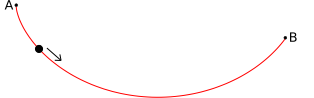
\includegraphics{brachistochrone.png}
\end{center}
}

%-------------------------------------------------------------------------------
%	CHAPTER 6
%-------------------------------------------------------------------------------

\chapter[Euler-Lagrange II]{The Euler-Lagrange equation, II:\\ Constraints}

Imposing constraints works in the infinite-dimensional theory just as well as it does in the finite-dimensional theory using the method of Lagrange multipliers. We will only consider constraints of the form
\[G(y)=\int_a^bM(x,y(x),y'(x))dx=0\]
for some Lagrangian $M(p,q,r)$.

\begin{exm}
Suppose we want to minimise the arc-length of the graph of $y\colon[a,b]\to\RR$ given that the area underneath the graph is equal to $K$. Now
\[A(y)=\int_a^b\sqrt{1+(y')^2}dx\]
is the arc-length and
\[G(y)=\int_a^b\left(y-\frac{K}{b-a}\right)dx\]
measures how far the area underneath the graph is from $K$. We introduce a Lagrange multiplier $\lambda$ and minimise the functional
\[F(y,\lambda)=\int_a^b\left(\sqrt{1+(y')^2}-\lambda\left(y-\frac{K}{b-a}\right)\right)dx.\]
Varying with respect to $\lambda$ gives us the constraint $G(y)=0$ (i.e. the area under the graph of $y$ is $K$) and with respect to $y$ gives the Euler-Lagrange equation
\[-\lambda=\frac{d}{dx}\frac{y'}{\sqrt{1+(y')^2}}\]
so
\[y'=\frac{D-\lambda x}{\sqrt{1-(D-\lambda x)^2}}.\]
Using $D-\lambda x=\sin\theta$ we get $\lambda y+C=\cos\theta$ for some constant $C$, so
\[(\lambda y +C)^2+(D-\lambda x)^2=1\]
and the graph $(x,y(x))$ lies on a circle of radius $1/\lambda$ (it is a segment of circle between $(a,y_a)$ and $(b,y_b)$).

We could also have used Beltrami's identity.
\end{exm}
\begin{exm}[Catenary]
Consider a chain hanging above the $x$-axis with its endpoints fixed at $(a,y_a)$, $(b,y_b)$. It will hang so as to minimise its total potential energy. If the chain is uniform with density $\rho\ kg m^{-1}$ then the segment lying over an infinitesimal segment $dx$ has mass $\rho\sqrt{1+(y')^2}dx$. The potential energy of this segment is $\rho gy\sqrt{1+(y')^2}dx$ so the functional to be minimised is
\[A(y)=\rho g\int_a^by\sqrt{1+(y')^2}dx.\]
However, the chain is inelastic so its length is fixed at $K$ metres
\[G(y)=\int_a^b\left(\sqrt{1+(y')^2}-\frac{K}{b-a}\right)dx=0.\]
The modified functional for the constrained problem is
\[\int_a^b\left(\rho gy\sqrt{1+(y')^2}-\lambda\left(\sqrt{1+(y')^2}-\frac{K}{b-a}\right)\right)dx\]
which has no explicit $x$-dependence, so we will solve this constrained problem using Beltrami's identity.

Beltrami's identity implies
\[\rho gy\sqrt{1+(y')^2}-\lambda\left(\sqrt{1+(y')^2}-\frac{K}{b-a}\right)-y'(\rho gy-\lambda)y'/\sqrt{1+(y')^2}=c\]
for some constant $c$. This gives
\[\rho gy-\lambda=\left(c-\lambda K/(b-a)\right)\sqrt{1+(y')^2}.\]
We define $C:=c-\lambda K/(b-a)$ and we rearrange to get
\[y'=\sqrt{(\rho gy-\lambda)^2/C^2-1}.\]
Substituting $\cosh z=(\rho gy-\lambda)/C$ we integrate and get
\[x=\frac{C}{\rho g}\cosh^{-1}\frac{\rho gy-\lambda}{C}-D\]
or
\[y=\frac{C}{\rho g}\cosh\left(\frac{\rho g}{c}(x+D)\right)+\frac{\lambda}{\rho g}.\]
This curve is called the {\em catenary curve} from the Latin ``catena'' meaning chain. It is the same as the curve whose surface of revolution (catenoid) minimises surface area.
\end{exm}

%-------------------------------------------------------------------------------
%	CHAPTER 7
%-------------------------------------------------------------------------------

\chapter[Euler-Lagrange, III]{The Euler-Lagrange equation, III:\\ More variables}

\section{Vector-valued functions}

We have already seen an example (action of a curve in the plane) where the functions of interest are vector-valued.

\begin{thm}
Let $V$ be the space of functions $\vec{y}\colon [a,b]\to\RR^n$ satisfying the boundary conditions $\vec{y}(a)=\vec{y}_a$ and $\vec{y}(b)=\vec{y}_b$. We will write $\vec{y}(x)$ in coordinates $(y_1(x),\ldots,y_n(x))$. Let $A$ be a functional defined by a Lagrangian $L(p,q_1,\ldots,q_n,r_1,\ldots,r_n)$ by
\[A(\vec{y})=\int_a^bL(x,y_1(x),\ldots,y_n(x),y'_1(x),\ldots,y'_n(x))dx.\]
Let $\vec{\epsilon}(x)$ be a function such that $\vec{\epsilon}(a)=\vec{\epsilon}(b)=0$. Then the G\^{a}teaux derivative of $A$ at $\vec{y}$ in the $\vec{\epsilon}$ direction is
\[d_{\vec{y}}A(\vec{\epsilon})=\sum_{i=1}^n\int_0^1\left(\frac{\partial L}{\partial y_i}-\frac{d}{dx}\frac{\partial L}{\partial y'_i}\right)\epsilon_i(x)dx\]
which vanishes for all $\vec{\epsilon}$ if and only if the $n$ Euler-Lagrange equations hold
\[\frac{\partial L}{\partial y_i}-\frac{d}{dx}\frac{\partial L}{\partial y'_i}=0,\qquad i=1,\ldots,n.\]
\end{thm}
The proof is so similar to the proof for functions $y\colon[a,b]\to\RR$ that I will omit it.

\subsection{Examples}

\begin{exm}[Isoperimetric problem]
Let $\gamma\colon\RR\to\RR^2$ be a curve with coordinates $\gamma(t)=(x(t),y(t))$. We assume that $\gamma$ is a closed curve ($\gamma(t+2\pi)=\gamma(t)$ which is just as good for integrating by parts as assuming $\gamma(0)$ and $\gamma(1)$ are fixed. Suppose that we know it has action $\int_0^1{2\pi}(\dot{x}^2+\dot{y}^2)dt=K$ and we want to maximise the area of the region it bounds.

By Green's theorem, the area of this region $U$ is
\[\int_Udxdy=\int_{\partial U}xdy\]
or
\[\int_0^{2\pi}x(t)\dot{y}(t)dt.\]
Therefore we must find the critical points of the constrained problem
\[\int_0^{2\pi}\left(x\dot{y}-\lambda\left(\dot{x}^2+\dot{y}^2-K/2\pi\right)\right)dt.\]
The two Euler-Lagrange equations are
\begin{align*}
\dot{y}&=\frac{d}{dt}\left(-2\lambda\dot{x}\right)\\
0&=\frac{d}{dt}\left(x-2\lambda\dot{y}\right).
\end{align*}
This gives
\[\ddot{x}=-\dot{y}/2\lambda,\qquad\ddot{y}=\dot{x}/2\lambda.\]
Differentiating again allows us to rearrange and obtain
\[\dddot{y}=-\dot{y}/4\lambda^2,\qquad\dddot{x}=-\dot{x}/4\lambda^2\]
so $\dot{x}$ and $\dot{y}$ obey simple harmonic motion. This means that $t\mapsto(x(t),y(t))$ is a circle.
\end{exm}

\section{Functions of several variables}

Now let $U\subset\RR^m$ be an open subset whose boundary $\partial U$ is smooth. We will consider functions $\phi\colon U\to\RR$ with fixed boundary values; in other words we will fix a function $\phi_0\colon\partial U\to\RR$ and consider functions $\phi$ such that
\[\phi(\vec{x})=\phi_0(\vec{x}),\qquad\vec{x}\in\partial U.\]
Perturbations $\epsilon(\vec{x})$ satisfy $\epsilon(\vec{x})=0$ for $\vec{x}\in\partial U$. Our Lagrangian $L$ will now depend on $\vec{x}=(x_1,\ldots,x_m)$, on $\phi(\vec{x})$ and on the partial derivatives $\partial_i\phi=\frac{\partial \phi}{\partial x_i}$, $i=1,\ldots,m$, that is:
\[A(\vec{y})=\int_UL\left(\vec{x},\phi(\vec{x}),\nabla\phi(\vec{x})\right)dx_1\cdots dx_m\]

\begin{thm}
The G\^{a}teaux derivative of $A$ at $\phi$ in the $\epsilon$-direction is
\[d_{\phi}A(\epsilon)=\int_0^1\left(\frac{\partial L}{\partial \phi}-\sum_{i=1}^m\frac{\partial}{\partial x_i}\frac{\partial L}{\partial(\partial_i\phi)}\right)\epsilon(x)dx\]
which vanishes for all $\epsilon$ if and only if the Euler-Lagrange equation holds
\[\frac{\partial L}{\partial\phi}-\sum_{i=1}^m\frac{\partial}{\partial x_i}\frac{\partial L}{\partial (\partial_i\phi)}=0.\]
\end{thm}
\begin{proof}
Let $t\epsilon$ be a small perturbation of $\phi$. By the chain rule, we have
\[\left.\frac{d}{dt}\right|_{t=0}L(\phi+t\epsilon)=\epsilon\frac{\partial L}{\partial\phi}+\sum_{i=1}^m(\partial_i\epsilon)\frac{\partial L}{\partial(\partial_i\phi)}.\]
Integrating this over $U$ gives the G\^{a}teaux derivative
\[d_{\phi}A(\epsilon)=\int_U\left(\epsilon\frac{\partial L}{\partial\phi}+\sum_{i=1}^m(\partial_i\epsilon)\frac{\partial L}{\partial(\partial_i\phi)}\right)dx_1\cdots dx_m\]
The last term can be written $\nabla\epsilon\cdot\frac{\partial L}{\partial(\nabla\phi)}$ where $\frac{\partial L}{\partial(\nabla\phi)}$ denotes the vector whose $i$th component is $\frac{\partial L}{\partial(\partial_i\phi)}$.

We have
\[\nabla\cdot\left(\epsilon\frac{\partial L}{\partial(\nabla\phi)}\right)=\nabla\epsilon\cdot\frac{\partial L}{\partial(\nabla\phi)}+\epsilon\nabla\cdot\frac{\partial L}{\partial(\nabla\phi)}=\sum_{i=1}^m\left(\partial_i\epsilon\frac{\partial L}{\partial(\partial_i\phi)}+\epsilon\frac{\partial}{\partial x_i}\frac{\partial L}{\partial(\partial_i\phi)}\right).\]
Integrating this over $U$ and applying Stokes's theorem gives
\[\int\nabla\epsilon\cdot\frac{\partial L}{\partial(\nabla\phi)}dx_1\cdots dx_m=-\int_{\partial U}\epsilon\frac{\partial L}{\partial(\nabla\phi)}\cdot\hat{\vec{n}}dS\]
where $\hat{\vec{n}}$ is the outward normal to $\partial U$ and $dS$ is the volume element on $\partial U$. This vanishes because $\epsilon$ vanishes on $\partial U$. Therefore
\[\int_U\nabla\epsilon\cdot\frac{\partial L}{\partial(\nabla\phi)}dx_1\cdots dx_m=-\int_U\epsilon\nabla\cdot\frac{\partial L}{\partial(\nabla\phi)}=-\int_U\sum_{i=1}^m\epsilon\frac{\partial}{\partial x_i}\frac{\partial L}{\partial(\partial_i\phi)}\]
which is the analogue of integration by parts in several variables. This allow us to deduce
\[d_{\phi}A(\epsilon)=\int_U\left(\frac{\partial L}{\partial\phi}-\nabla\cdot\frac{\partial L}{\partial(\nabla\phi)}\right)\epsilon dx_1\cdots dx_m.\]
The fundamental theorem of the calculus of variations in several variables\footnote{This is proved in the same way as the one-variable case but using a bump-function in several variables - this can be taken to be the usual bump function applied to the radius $\sqrt{\sum_{i=1}^mx_i^2}$.} states that this vanishes for all $\epsilon$ if and only if
\[\frac{\partial L}{\partial\phi}-\nabla\cdot\frac{\partial L}{\partial(\nabla\phi)}=0.\]
Unwinding the definition of $\partial L/\partial(\nabla\phi)$ gives the formulae in the statement of the theorem.
\end{proof}
\begin{rmk}
The Euler-Lagrange equation is now a second-order \emph{partial} differential equation.
\end{rmk}

\subsection{Examples}

\begin{exm}
Consider $U=[0,1]^2$, the square, and functions $\phi$ with fixed boundary values
\begin{align*}
\phi(x,0)&=\phi_0(x,0),&\phi(x,1)&=\phi_0(x,1),\\
\phi(0,y)&=\phi_0(0,y),&\phi(1,y)&=\phi_0(1,y).
\end{align*}
We will try to minimise the functional
\[A(\phi)=\int_0^1\int_0^1\left(\left(\frac{\partial\phi}{\partial x}\right)^2+\left(\frac{\partial\phi}{\partial y}\right)^2\right)dx dy.\]
We can think of this functional as the total gradient $\int|\nabla\phi|^2dxdy$ of a temperature distribution $\phi$ on $U$. Since heat flows to minimise a gradient, a minimiser for this functional will be a steady-state temperature distribution on the square.

We have
\[\frac{\partial L}{\partial \phi}=0\qquad\frac{\partial L}{\partial(\partial_x\phi)}=2\partial_x\phi,\qquad\frac{\partial L}{\partial(\partial_y\phi)}=2\partial_y\phi\]
so the Euler-Lagrange equation is
\[\frac{\partial^2\phi}{\partial x^2}+\frac{\partial^2\phi}{\partial y^2}=0.\]
This is called Laplace's equation and will be important later in the course.
\end{exm}
\begin{exm}
Now let us use the functional
\[A(\phi)=\int_U\sqrt{1+(\partial_x\phi)^2+(\partial_y\phi)^2}dx dy.\]
This measures the area of the graph\footnote{To see this, note that the two vectors $(1,0,\partial_x\phi)$ and $(0,1,\partial_y\phi)$ are tangent to the graph of $\phi$ and they span a parallelogram with area $\sqrt{1+(\partial_x\phi)^2+(\partial_y\phi)^2}$. The infinitesimal area element living over $dx dy$ is therefore an infinitesimal parallelogram of area $\sqrt{1+(\partial_x\phi)^2+(\partial_y\phi)^2}dxdy$.} of $\phi$. The Euler-Lagrange equation is 
\[\frac{\partial L}{\partial\phi}=\frac{\partial}{\partial x}\frac{\partial L}{\partial\phi_x}+\frac{\partial}{\partial y}\frac{\partial L}{\partial\phi_y}\]
and in this case
\[L=\sqrt{1+\phi_x^2+\phi_y^2}\]
so
\begin{align*}
0&=\frac{\partial}{\partial x}\frac{\phi_x}{\sqrt{1+|\nabla\phi|^2}}+\frac{\partial}{\partial y}\frac{\phi_y}{\sqrt{1+|\nabla\phi|^2}}\\
&=\frac{\Delta\phi}{\sqrt{1+|\nabla\phi|^2|}}-\frac{\phi_x(\phi_x\phi_{xx}+\phi_y\phi_{yy})+\phi_y(\phi_y\phi_{yy}+\phi_x\phi_{xy})}{(1+|\nabla\phi|^2)^{3/2}}\\
&=\frac{1}{(1+|\nabla\phi|^2)^{3/2}}\left(\phi_{xx}(1+\phi_y^2)+\phi_{yy}(1+\phi_x^2)-2\phi_x\phi_y\phi_{xy}\right)
\end{align*}
(remember that $\nabla\phi=(\phi_x,\phi_y)$ and $\Delta\phi=\phi_{xx}+\phi_{yy}$). This gives us the equation for a {\em minimal surface}:
\[\frac{\partial^2\phi}{\partial x^2}\left(1+\left(\frac{\partial\phi}{\partial y}\right)^2\right)+\frac{\partial^2\phi}{\partial y^2}\left(1+\left(\frac{\partial\phi}{\partial x}\right)^2\right)=2\frac{\partial\phi}{\partial x}\frac{\partial\phi}{\partial y}\frac{\partial^2\phi}{\partial x\partial y}.\]
\end{exm}

%%% Local Variables: 
%%% mode: latex
%%% TeX-master: "notes"
%%% End: 